\documentclass[14pt]{extarticle}
\usepackage[utf8]{inputenc}
\usepackage[T1]{fontenc}
\usepackage[spanish,es-lcroman]{babel}
\usepackage{amsmath}
\usepackage{amsthm}
\usepackage{physics}
\usepackage{tikz}
\usepackage{float}
\usepackage{calc}
\usepackage[autostyle,spanish=mexican]{csquotes}
\usepackage[per-mode=symbol]{siunitx}
\usepackage{gensymb}
\usepackage{multicol}
\usepackage{enumitem}
\usepackage{setspace}
\usepackage[left=2.00cm, right=2.00cm, top=2.00cm, 
     bottom=2.00cm]{geometry}
\usepackage{Estilos/ColoresLatex}
\usepackage{makecell}
\usepackage{subcaption}

% \usepackage[sfdefault]{roboto}  %% Option 'sfdefault' only if the base font of the document is to be sans serif
% \usepackage[T1]{fontenc}

\usepackage{scalerel}[2016-12-29]
\def\stretchint#1{\vcenter{\hbox{\stretchto[440]{\displaystyle\int}{#1}}}}
\def\scaleint#1{\vcenter{\hbox{\scaleto[3ex]{\displaystyle\int}{#1}}}}
\def\bs{\mkern-12mu}

\newcommand{\textocolor}[2]{\textbf{\textcolor{#1}{#2}}}
\sisetup{per-mode=symbol}
\decimalpoint
\sisetup{bracket-numbers = false}
\newlength{\depthofsumsign}
\setlength{\depthofsumsign}{\depthof{$\sum$}}
\newcommand{\nsum}[1][1.4]{% only for \displaystyle
    \mathop{%
        \raisebox
            {-#1\depthofsumsign+1\depthofsumsign}
            {\scalebox
                {#1}
                {$\displaystyle\sum$}%
            }
    }
}

\title{\vspace*{-2cm} Difracción}
\date{ }

\begin{document}
\maketitle

\section{Difracción.}

Ya se revisó que un tren de ondas no se puede acortar sin que se disperse en una multitud de frecuencias. De forma similar un frente de onda no se puede acortar en extensión transversal mediante diafragmas sin que se esparza en varias direcciones. Al primer fenómeno se le podría llamar \textit{difracción temporal} y al segundo \textit{difracción espacial}. Sin embargo, al segundo se le llama simplemente \underline{\textit{difracción}} y se ilustra en la figura (\ref{fig:figura_X_01}).
\begin{figure}[H]
    \centering
    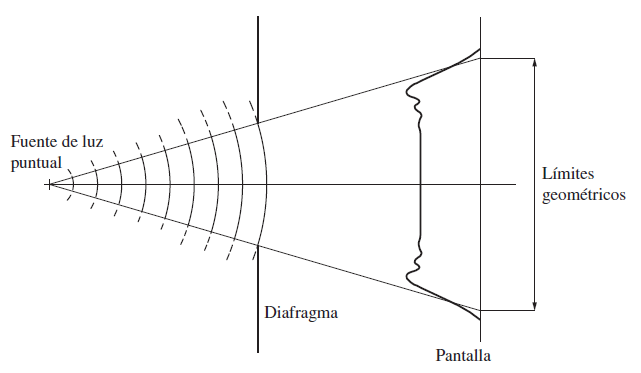
\includegraphics[scale=0.75]{Imagenes/Difraccion_01.png}
    \caption{Difracción de la luz.}
    \label{fig:figura_X_01}
\end{figure}
Como se puede ver, llega luz a la pantalla fuera de los límites de la sombra geométrica debido a este fenómeno que ahora estudiaremos. El fenómeno fue observado por primera vez en 1665 por Francesco Maria Grimaldi, quien acuñó el término difracción.

\subsection{Principio de Huygens.}

A fin de poder explicar la difracción, Christiaan Huygens propuso en los Países Bajos la regla de que \enquote{cada punto de un frente de onda se considere como una nueva fuente de ondas esféricas}. Éste es el llamado \textbf{principio de Huygens}, que se puede ilustrar por medio de la figura (\ref{fig:figura_X_02}).
\begin{figure}[H]
    \centering
    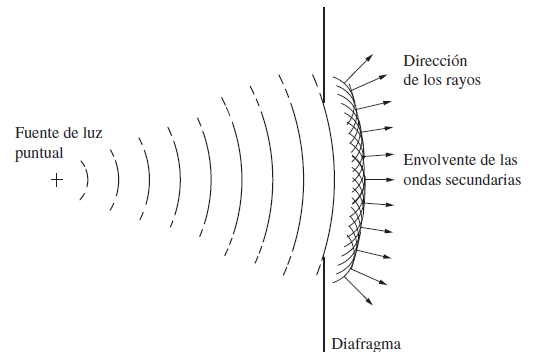
\includegraphics[scale=0.75]{Imagenes/Difraccion_02.png}
    \caption{Principio de Huygens para explicar la difracción.}
    \label{fig:figura_X_02}
\end{figure}
Según Huygens, las ondas secundarias, después de pasar por la abertura, se suman produciendo un nuevo frente de onda que casi coincide con la envolvente de dichas ondas secundarias. Esta suma de las ondas secundarias es tal que en un punto sobre su envolvente se cancelan entre sí los efectos laterales quedando sólo los que tienen la dirección de propagación de la onda. Sin embargo, esta cancelación no puede ocurrir cerca de la orilla de la obstrucción, razón por la cual la onda se esparce en varias direcciones. De esta forma se puede explicar que la luz se desvíe en las cercanías de la orilla de la abertura hacia zonas dentro de la sombra geométrica, pero no se puede sin embargo explicar el hecho de que aparezcan franjas de interferencia en las cercanías de la sombra.

Augustin-Jean Fresnel modificó esta teoría más de un siglo después de que Huygens la propusiera, suponiendo que los frentes de onda secundarios no solamente se unían para formar una envolvente del frente de onda, sino que además interferirían unos con otros según los principios de la interferencia que se describieron en el capítulo anterior. Dicho de otro modo, los disturbios ópticos debidos a cada frente de onda secundario deben sumarse sobre la pantalla iluminada, tomando en cuenta su amplitud y fase en cada punto. El principio de Huygens aplicado de esta manera se conoce con el nombre de principio de Huygens-Fresnel. Esta forma de explicar la difracción tiene bastante éxito, ya que puede dar cuenta exacta de las intensidades sobre la pantalla en que se observa la difracción, incluyendo la presencia de las franjas. Sin embargo, esta teoría tiene dos defectos, uno es que no puede explicar por qué las ondas esféricas secundarias se propagan solamente en la dirección de la onda primaria y no hacia atrás. El otro es que no se obtiene con ella resultados correctos para la fase de la onda sobre la pantalla, sino desviados 90° con respecto a su valor real. Estas deficiencias fueron eliminadas por Kirchhoff en 1876, quien llegó esencialmente a obtener las mismas ondas secundarias que Huygens, pero en esta teoría aparecen como contribuciones diferenciales del frente de onda. No obstante, la teoría de Kirchhoff que se describirá en la siguiente sección aún es incompleta a pesar de obtener resultados sorprendentemente aproximados a la realidad. Los resultados exactos sólo se obtienen usando la teoría electromagnética.

\subsection{Teoría de la difracción de Kirchhoff.}
 
En 1876 Kirchhoff demostró que la teoría intuitiva pero muy eficaz de Huygens-Fresnel se puede justificar con un teorema integral basado en la ecuación de onda que ya estudiamos al inicio del curso. Para explicar brevemente la teoría desarrollada

\end{document}